\documentclass{beamer}
\usepackage[utf8]{inputenc}
\usepackage{url,hyperref,times}
\usepackage[T1]{fontenc}
\usepackage{verbatim,scalefnt,colortbl}
\usepackage[spanish]{babel}
\usepackage{graphics}
\mode<presentation>
{
   \usetheme{CambridgeUS}
%   \usetheme{Berkeley}
%  \usetheme{Madrid}

  \setbeamercovered{transparent}
  \setbeamertemplate{navigation symbols}{}
  \setbeamertemplate{footline}[page number]{}
  \usebackgroundtemplate{
\includegraphics[width=128mm, heigth=96mm]{dna-strand-code.jpg}}
  \setbeamercolor{normal text}{fg=black}
}
\usefonttheme{structureitalicserif}
\begin{document}
\title[]{Whole genome alignment in High Performance Computing environments}
\author[Julio García]{Julio César García Vizcaíno \and Directores: Antonio Espinosa, Juan Carlos Moure}
\institute[UAB]{
   
\includegraphics[scale=0.4]{caos.jpg}\\
   Computer Architecture \& Operating Systems Department\\
   Universitat Autónoma de Barcelona
}
\date[\today]{\today}
\pgfdeclareimage[height=0.3cm, width=0.6cm]{uab-logo.jpg}{uab-logo.jpg}
\logo{\pgfuseimage{uab-logo.jpg}}

\begin{frame}
  \titlepage
\end{frame}
\begin{frame}
  \frametitle{Contents}\tableofcontents
\end{frame}
\section{Problem definition}
\begin{frame}
  \frametitle{Whole Genome Alignment in MUMmer}
  \begin{figure}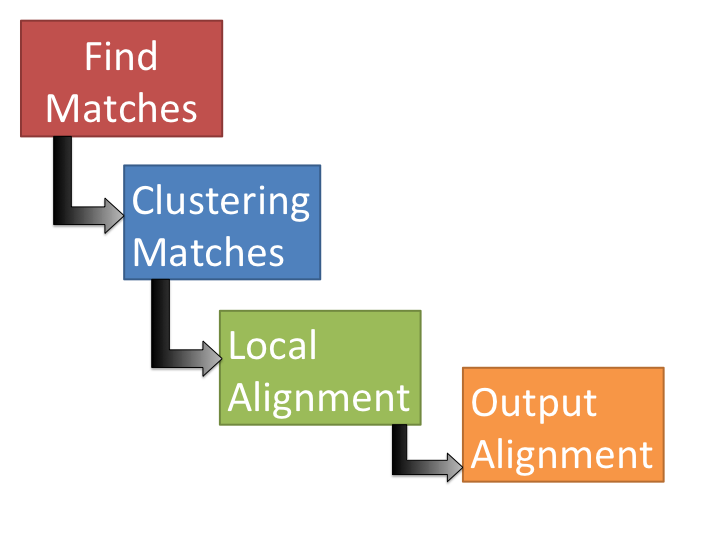
\includegraphics[scale=0.4]{wga.png}\end{figure}
\end{frame}
\begin{frame}
\frametitle{Search of Maximal Unique Matches}
\begin{figure}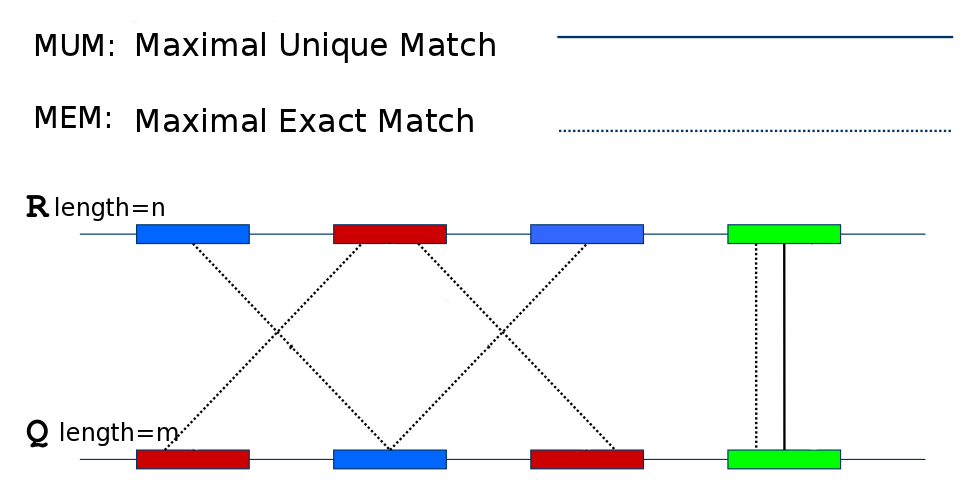
\includegraphics[scale=0.25]{mem-mum.png}\end{figure}
\begin{figure}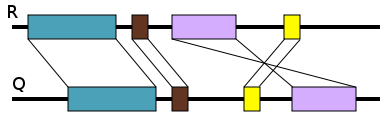
\includegraphics[scale=0.555555]{mums.png}\end{figure}
\end{frame}
\begin{frame}
\frametitle{Genome alignment: search of Maximal Unique/Exact Matches}
\begin{figure}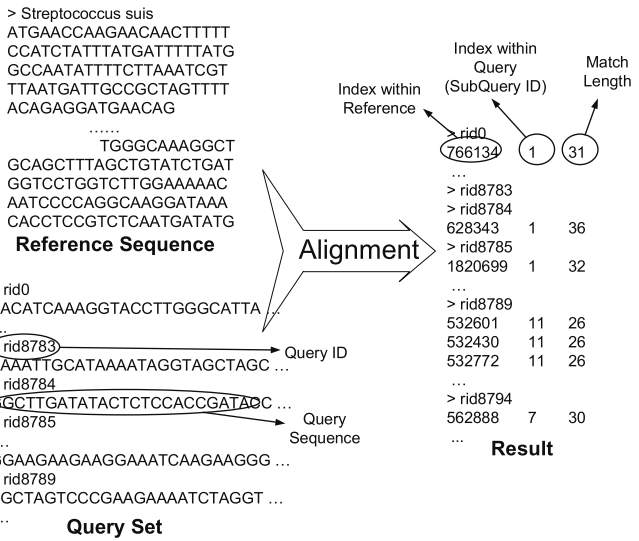
\includegraphics[scale=0.35]{problem.png}\end{figure}
\end{frame}
\begin{frame}[fragile]
  \frametitle{Traversal of suffix tree}
  \begin{block}{Search of MUMs}
  \begin{figure}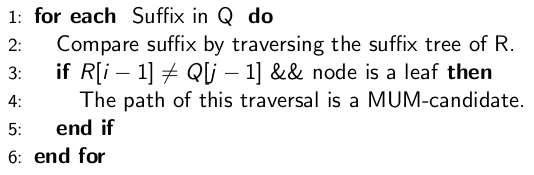
\includegraphics[scale=0.4]{algoritmo.png}\end{figure}
  \end{block}
  \begin{figure}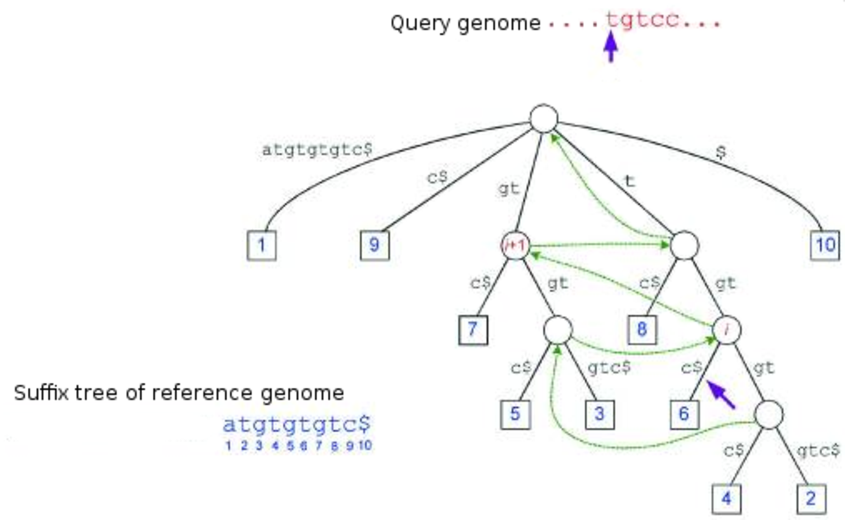
\includegraphics[scale=0.4]{st-mum.pdf}\end{figure}
\end{frame}
%\begin{frame}
%  \frametitle{Find MUM in suffix tree}
%  \begin{figure}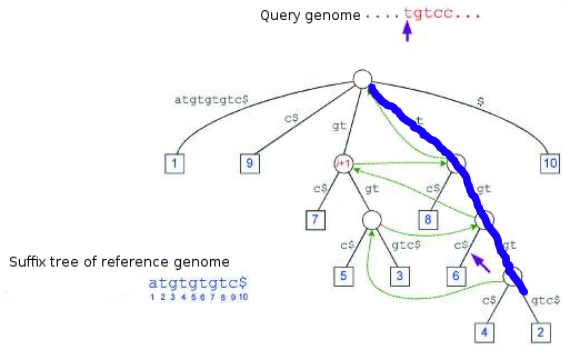
\includegraphics[scale=0.8]{mum.png}\end{figure}
%\end{frame}
\section{Objectives}
\begin{frame}
 \frametitle{General objective}
 \begin{block}{General objective}
Speed up the search of exact matches (distributed) considering the use of computer and memory resources; and adapt it to application MUMmer for its execution in HPC cluster multicore environments.
\end{block}
\end{frame}
\begin{frame}
  \frametitle{Search of MUMs in Multicore architectures}
  \begin{figure}
    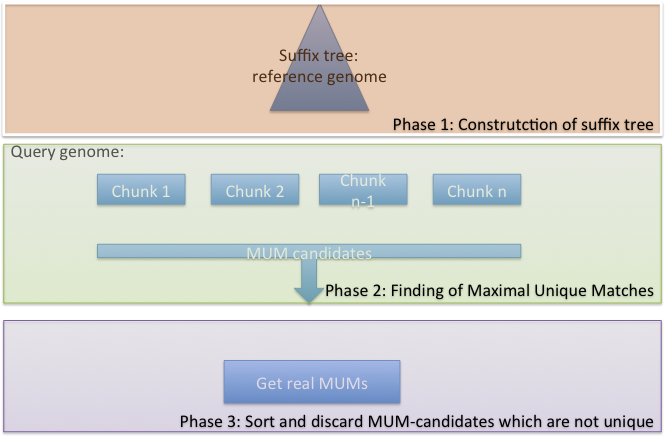
\includegraphics[scale=0.45]{Phases.png}
  \end{figure}
\end{frame}
\section{Parallel search of maximal unique matches}
%\begin{frame}
%  \frametitle{Distributed and parallel search of maximal matches}
%  \begin{block}{Split query sequence}
%    Consider a query sequence of length $n$ and a distributed suffix tree. How to find the maximal matches of query sequence: acaccacaaccaacaaaaccaccacacc in distributed suffix tree?
% \end{block}
%\end{frame}
\begin{frame}
  \frametitle{Parallel search of maximal unique matches}
  \begin{block}{}
\begin{itemize}
\item Hardware:  
\begin{itemize}
\item 2 Processor Intel(R) Xeon(R) E5645 @ 2.4GHz of 6 cores each one, 32KB L1 cache, 256KB L2 and 12MB L3 shared cache per socket.
\item RAM: 96 GB
\end{itemize} 
\item  Software: 
\begin{itemize}
\item Linux Kernel 2.6.32-220.el6.x86\_64 \#1 SMP
\item gcc 4.7.0 with OpenMP support
\item PAPI 5.0.1
\end{itemize}  
\item Genomes:
  \begin{itemize}
    \item Reference: Human chromosome 21 single fasta file
    \item Query: Mouse chromosome 16 single fasta file
  \end{itemize}
\end{itemize}
  \end{block}
\end{frame}
\begin{frame}
  \frametitle{Parallel search of maximal unique matches}
  \begin{figure}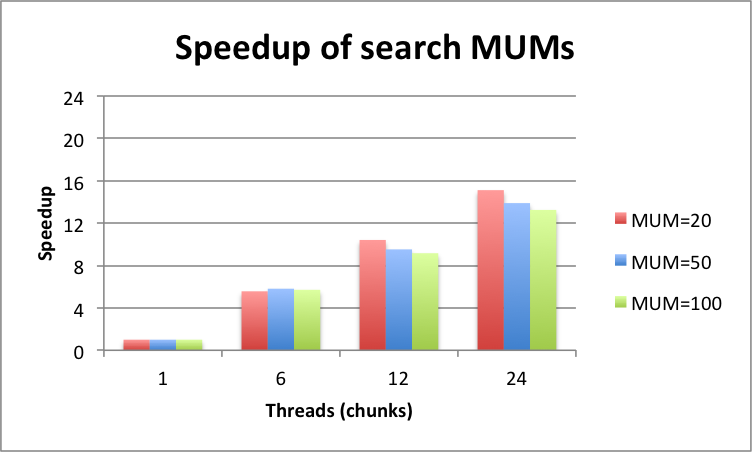
\includegraphics[scale=0.8]{speedup.png} \end{figure}
\end{frame}
  
\section{Conclusions}
    \begin{frame}
    \frametitle{Conclusions}
    \begin{block}{Current work}
      \begin{itemize}
        \item Evaluation of performance to search MUMs of a query and reference genome in multi-core architectures with OpenMP.
        \item Results shows that the heaviest section of searching MUMs in a suffix tree is improved with the use of a multi-core architecture. 
        \item Bottleneck is in suffix tree: traverse a suffix tree in multi-core architectures.
      \end{itemize}
\end{block}
\end{frame}
\begin{frame}
  \frametitle{Future work}
\begin{block}{}
Implement Distributed Suffix Tree.\\
Perform massive searches of maximal matches: design and test a parallel and distributed algorithm to perform the search of maximal matches in Distributed Suffix Tree for HPC multicore environments.
\end{block}
\end{frame}
\section{}
\begin{frame}
  \begin{center}
    \Huge{Thanks!}
\end{center}
\end{frame}
\begin{frame}
  \titlepage
\end{frame}
\end{document}
